\documentclass[conference]{IEEEtran}
%\IEEEoverridecommandlockouts
%\IEEEoverridecommandlockouts
% The preceding line is only needed to identify funding in the first footnote. If that is unneeded, please comment it out.
\usepackage{cite}
\usepackage{amsmath,amssymb,amsfonts}
\usepackage{diffcoeff}
\usepackage{isomath}
\usepackage{siunitx}
\usepackage{algorithmic}
\usepackage{graphicx}
\usepackage{textcomp}
\usepackage{xcolor}
\usepackage{tikz}
\newlength\imagewidth
\newlength\imagescale
\usepackage[nonumberlist,acronym,nomain]{glossaries}
\usepackage{cleveref}
%\usepackage{caption}
\usepackage[caption=false,font=footnotesize]{subfig}

\usepackage{algorithm}
\usepackage{algpseudocode}
\usepackage{float}


\floatstyle{plain}
% \usepackage[a4paper, total={6in, 8in}, left=1.8cm, right=1.8cm, top=1.8cm, bottom=2.9cm]{geometry}
% \usepackage{geometry}
%  \geometry{ a4paper, total={210mm,297mm}, left=17mm, right=17mm, top=22mm, bottom=32mm }
\setlength{\columnsep}{0.25in}
\def\BibTeX{{\rm B\kern-.05em{\sc i\kern-.025em b}\kern-.08em
    T\kern-.1667em\lower.7ex\hbox{E}\kern-.125emX}}

\DeclareMathOperator{\csch}{csch}
\newcommand{\e}{\ensuremath{\text{e}}}
\newcommand{\infint}{\ensuremath{\int_{\infty}^{\infty}}}
\newcommand{\hpoly}[2][n]{\ensuremath{\exp\left\{-\frac{{#2}^2}{2}\right\} H_{#1}\left(#2\right)}}
\newcommand{\hpolye}[2][n]{\ensuremath{\e^{-\frac{{#2}^2}{2}} H_{#1}\left(#2\right)}}
\newcommand{\hpolyp}[2][n]{\ensuremath{\exp\left\{-\frac{\left(#2\right)^2}{2}\right\} H_{#1}\left(#2\right)}}
\newcommand{\F}{\ensuremath{\mathcal{F}}}

\loadglsentries{acronyms.tex}
    
\begin{document}

\title{Measurement-Driven Latency Analysis of Uplink/Downlink Scheduling in DECT-2020 NR
% {\footnotesize \textsuperscript{*}Note: Sub-titles are not captured in Xplore and
% should not be used}
% \thanks{Identify applicable funding agency here. If none, delete this.}
 }

\author{\IEEEauthorblockN{Ashuqullah Alizai}
\IEEEauthorblockA{\textit{Aalen University of Applied Sciences} \\
Aalen, Germany \\
ashuqullah.alizai@hs-aalen.de\\ ORCID 0000-0002-7625-2330}
\and
\IEEEauthorblockN{Mohammad Reza Mousavi}
\IEEEauthorblockA{\textit{Aalen University of Applied Sciences} \\
Aalen, Germany \\
mohammad.mousavi@hs-aalen.de\\ ORCID 0000-0003-2521-2651}
\and
\IEEEauthorblockN{Stephan Ludwig}
\IEEEauthorblockA{\textit{Aalen University of Applied Sciences} \\
Aalen, Germany \\
stephan.ludwig@hs-aalen.de\\ORCID 0000-0002-0233-1706}
}

\maketitle

\begin{abstract}

\gls{nr} is an \gls{etsi}-standardized non-cellular radio technology targeting low-latency communication in private and industrial networks. While several studies have reported promising end-to-end latency figures for \gls{nr}, the contribution of \gls{ul}/\gls{dl} scheduling and hardware-induced direction switching to overall latency has not been thoroughly quantified in practical implementations. In this work, we present a measurement-driven latency analysis of \gls{ul} and \gls{dl} scheduling behavior in \gls{nr} star networks. Using oscilloscope and signal analyzer measurements on a single-chip \gls{nr} platform, we characterize the \gls{rx}--\gls{tx} turnaround delay associated with \gls{ul}/\gls{dl} alternation and evaluate its impact on end-to-end latency under different traffic and scheduling scenarios. The results show that, for short-packet and request--response traffic, turnaround-induced latency can constitute a significant portion of the total delay and is strongly influenced by scheduling decisions. Based on these observations, we discuss the limitations of scheduling-based mitigation on single-transceiver hardware and outline architectural directions, such as \gls{ul}/\gls{dl} channel separation, to further reduce latency in future \gls{nr} systems.
\end{abstract}



\begin{IEEEkeywords}
\gls{nr}, latency analysis, \gls{ul}/\gls{dl} scheduling, \gls{tdd} systems,  \gls{rx}-- \gls{tx} turnaround, star topology, measurement-based evaluation
\end{IEEEkeywords}

\section{Introduction}
% Motivation, problem statement, contributions
\gls{nr} is a non-cellular 5G radio technology designed to support  \gls{urllc} and \gls{mmtc} for private and industrial networks \cite{etsi_dect_nr_overview,perez_guirao_dect_nr_essentials}. By operating in unlicensed spectrum and supporting flexible deployment models, \gls{nr} enables local wireless networks that can be deployed and operated independently of mobile network operators. These properties make \gls{nr} attractive for latency-sensitive applications such as industrial automation, tactile Internet services, and real-time audio transmissions\cite{dect_live_audio_latency}.

Recent experimental studies have demonstrated that \gls{nr} can achieve sub-millisecond to few-millisecond end-to-end latency under favorable conditions \cite{dect_live_audio_latency,cheap_5g_dect_nr,silfur_dect_nr_performance}. These results confirm the potential of \gls{nr} for low-latency use cases and position it as a competitive alternative to both cellular and short-range wireless technologies. However, most existing evaluations focus on application-level or end-to-end latency metrics and treat the underlying radio and scheduling behavior as a black box.

In practical \gls{nr} implementations, cost and power constraints often motivate the use of a single transceiver chain in which \gls{ul} and \gls{dl} communication share the same RF and baseband hardware \cite{etsi_dect_nr_architecture}. As \gls{nr} relies on \gls{tdd}, \gls{ul} and \gls{dl} transmissions cannot occur simultaneously, and switching between transmission directions requires a finite reconfiguration interval. While the standard defines guard intervals to support such transitions, the actual  \gls{rx}-- \gls{tx} turnaround time is implementation-dependent and may introduce non-negligible latency, particularly for short-packet and request--response traffic patterns.

Although scheduling and \gls{ul}/\gls{dl} coordination have been widely studied in \gls{tdd}-based cellular systems to support  \gls{urllc} traffic \cite{tdd_scheduling_urllc}, comparatively little attention has been given to implementation-level turnaround effects in \gls{nr} systems. Existing \gls{nr} studies primarily rely on simulations or coarse-grained measurements and do not explicitly quantify the contribution of  \gls{rx}-- \gls{tx} switching delay or its interaction with scheduling behavior \cite{dect_mesh_performance,near_urllc_multihop_dect}. As a result, it remains unclear to what extent observed latency is fundamentally limited by hardware turnaround, scheduling decisions, or traffic characteristics.

Motivated by this gap, this paper presents a measurement-driven analysis of \gls{ul}/\gls{dl} latency in \gls{nr} star networks. Using oscilloscope measurements on a single-chip \gls{nr} platform, we characterize the  \gls{rx}-- \gls{tx} turnaround time and evaluate its contribution to end-to-end latency. We then analyze how current scheduling behavior influences the frequency and impact of direction switching and discuss potential mitigation strategies at the scheduling and architectural levels, including \gls{ul}/\gls{dl} channel separation. The goal of this work is not to propose a new scheduling algorithm, but to provide empirical insight into latency bottlenecks in practical \gls{nr} implementations and to inform future scheduler and hardware design choices.

%=============================Section Background====================================================%

\section{Background and Related Work}

\subsection{\gls{nr} Standardization and Design Goals}

\gls{nr}  is an \gls{etsi}-standardized non-cellular radio technology designed to support \gls{urllc} and \gls{mmtc} for private and industrial wireless networks \cite{etsi_dect_nr_overview}. By operating in unlicensed spectrum and supporting flexible deployment models, \gls{nr} enables localized wireless systems that can be deployed independently of mobile network operators. The standard specifies a \gls{tdd} physical layer with slot-based transmission and guard intervals intended to support \gls{ul} and \gls{dl} transitions \cite{etsi_dect_nr_architecture}. While these mechanisms are defined at a protocol level, implementation details such as transceiver reconfiguration and scheduling behavior are left open to vendors.

In addition to the \gls{etsi} specifications, several overview works describe \gls{nr} as a non-cellular 5G technology tailored for verticals such as industrial automation, smart infrastructure, and private IoT deployments \cite{perez_guirao_dect_nr_essentials}. These works emphasize the flexibility of \gls{nr} in terms of topology and spectrum usage, but they do not address implementation-level latency behavior.

\subsection{Experimental Evaluation of \gls{nr} Latency}

Recent experimental studies have demonstrated that \gls{nr} is capable of achieving low end-to-end latency under favorable conditions. Practical evaluations in the context of professional live audio transmission report sub-millisecond to few-millisecond latency using \gls{nr} hardware \cite{dect_live_audio_latency}. Similarly, work targeting tactile Internet and human-in-the-loop applications highlights the suitability of \gls{nr} for latency-critical communication, emphasizing its potential to meet  \gls{urllc} requirements \cite{cheap_5g_dect_nr}.

Academic performance evaluations further report low round-trip times and reliable communication in real deployments \cite{silfur_dect_nr_performance,bandara_dect_nr_latency}. These studies provide valuable insight into achievable latency figures and overall system performance. However, latency is typically reported as an aggregate metric, without detailed decomposition into scheduling delay, transceiver turnaround time, or other implementation-level contributors.

\subsection{Scheduling and \gls{ul}/\gls{dl} Coordination}

\gls{ul} and \gls{dl} scheduling has been widely studied in \gls{tdd}-based wireless systems, particularly in the context of 5G cellular networks supporting  \gls{urllc} traffic. Prior work shows that frame coordination and scheduling decisions play a crucial role in minimizing latency and avoiding excessive direction switching overhead \cite{tdd_scheduling_urllc}. These studies demonstrate that even when physical-layer transmission times are short, scheduling-induced delays can dominate end-to-end latency.

In \gls{nr} systems, scheduling and resource allocation are intentionally flexible to support a wide range of deployment scenarios \cite{etsi_dect_nr_architecture}. System-level \gls{nr} studies primarily focus on routing, scalability, and multi-hop performance in mesh topologies \cite{dect_mesh_performance,near_urllc_multihop_dect}. While these works address important networking aspects, they do not explicitly analyze the impact of \gls{ul}/\gls{dl} alternation and transceiver turnaround on latency in star-based or single-hop deployments.

\subsection{Summary and Research Gap}
In summary, existing literature establishes that \gls{nr} is capable of supporting low-latency communication and highlights the importance of scheduling in \gls{tdd}-based systems. However, there is limited measurement-driven analysis of \gls{ul}/\gls{dl} turnaround latency in practical \gls{nr} implementations, particularly on single-chip platforms where  \gls{rx} and  \gls{tx} share the same transceiver hardware. Moreover, the interaction between scheduling behavior and hardware-induced turnaround delay has not been explicitly quantified. This work addresses this gap by providing time-domain measurements of  \gls{rx}-- \gls{tx} turnaround latency and by analyzing its impact on \gls{ul}/\gls{dl} scheduling in \gls{nr} star networks.

%=============================Section System Model and Experimental Setup====================================================%

\section{System Model and Experimental Setup}
This section describes the considered system model, network topology, and hardware assumptions used throughout this work. The focus is on a practical industrial deployment of \gls{nr}, where a central controller coordinates latency-sensitive sensor and actuator traffic.

\subsection{Industrial Sensor--Actuator Star Topology}

We consider an industrial sensor--actuator network organized in a star topology, as illustrated in Fig.~\ref{fig:system_model}. The network consists of a central programmable logic controller (\gls{plc}) acting as the \gls{nr} fixed termination (\gls{ftnode}), multiple sensors (S1--S4), and multiple actuators (A1--A4). All wireless communication is coordinated by the \gls{ftnode}, and direct communication between sensors and actuators is not supported.

Sensors periodically or event-wise transmit measurement data to the \gls{plc} in the \gls{ul} direction, while actuators receive control commands from the \gls{plc} in the \gls{dl} direction. This communication pattern is representative of typical industrial automation scenarios, where sensing and actuation are tightly coupled through a central control entity. The star topology minimizes hop count and simplifies coordination, but concentrates \gls{ul} and \gls{dl} traffic at the \gls{plc}.

\begin{figure}[t]
\centering
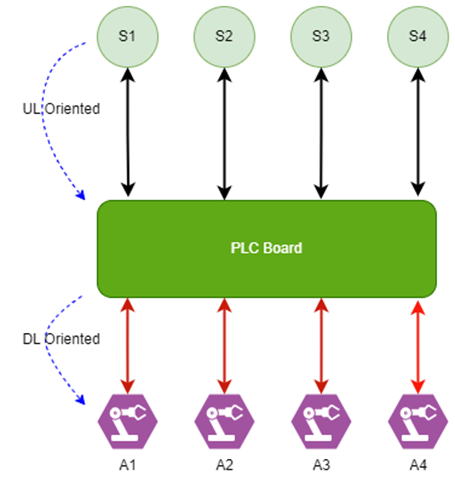
\includegraphics[width=0.9\linewidth]{SandAC.png}
\caption{Industrial sensor--actuator communication model based on an \gls{nr} star topology. 
Sensors (S1--S4) transmit measurement data to a central \gls{plc} acting as the \gls{nr} fixed termination (\gls{ftnode}) in the \gls{ul}, while actuators (A1--A4) receive control commands in the \gls{dl}. 
\gls{ul} and \gls{dl} transmissions alternate in time due to the use of a single  \gls{rx}/\gls{tx} transceiver at the \gls{plc}.}
\label{fig:system_model}
\end{figure}

\subsection{Duplexing and Communication Model}

\gls{nr} operates using \gls{tdd}, in which \gls{ul} and \gls{dl} transmissions share the same frequency resources and are separated in time. As a result, the system alternates between \gls{ul}-oriented phases, dominated by sensor data transmissions, and \gls{dl}-oriented phases, dominated by actuator command delivery.

In the considered system model, the \gls{plc} /\gls{ftnode} cannot transmit and receive simultaneously. Instead, it switches between  \gls{rx} and \gls{tx} states depending on the current scheduling decision. Guard intervals are used to support these transitions; however, the duration of the \gls{rx}--\gls{tx} switching process is implementation-dependent and not explicitly defined by the \gls{nr} standard.

\subsection{Hardware Assumptions}

The system model assumes a practical \gls{nr} implementation based on the Nordic Semiconductor nRF9151 system-on-chip, which integrates the radio-frequency front-end, baseband processing, and protocol stack on a single device. In this platform, transmission and reception share a single RF transceiver chain, preventing simultaneous \gls{rx} and \gls{tx} operation.

Consequently, each transition between \gls{ul} and \gls{dl} communication requires a hardware and firmware reconfiguration of the transceiver, resulting in a finite \gls{rx}--\gls{tx} turnaround delay. This delay is influenced by the internal radio state machine, firmware processing, and timing alignment with the \gls{nr} frame structure. While the \gls{nr} standard specifies guard intervals to support direction switching, the exact turnaround duration is implementation-dependent and not explicitly defined by the standard.

The nRF9151-based architecture reflects a class of cost- and power-efficient embedded \gls{nr} platforms commonly used in industrial and private network deployments. As such, the observed turnaround behavior is representative of practical single-transceiver \gls{nr} implementations rather than an artifact of a specific experimental setup.

\subsection{Scheduling Scope and Latency Components}

This work does not assume a specific scheduling algorithm; instead, it analyzes the observable scheduling behavior and its interaction with \gls{rx}--\gls{tx} switching under different \gls{ul}/\gls{dl} transmission scenarios. Higher-layer protocols, multi-hop routing, and mesh networking are outside the scope of this study.

Based on the above assumptions, the end-to-end latency experienced by sensor and actuator traffic can be decomposed into three main components: (i) scheduling and queuing delay at the \gls{mac} layer, (ii) \gls{rx}--\gls{tx} turnaround delay caused by transceiver reconfiguration, and (iii) physical-layer transmission time. The primary focus of this paper is on quantifying the turnaround-related component and evaluating how \gls{ul}/\gls{dl} scheduling decisions influence its impact on latency.


\subsection{Experimental Setup }

Fig.~\ref{fig:setup} shows the complete laboratory measurement setup. The turnaround delay is measured using GPIO timing markers captured on the \gls{dso}. In our measurements, the LTE/DECT RF ports were connected to laboratory instruments (e.g., oscilloscope) to monitor RF activity and, in some runs, to provide a controlled termination. Consequently, radiated power is strongly attenuated, and the two nodes communicate only at very short range, mainly via leakage coupling around the RF connectors and nearby cables. The setup is intended to study timing and scheduling effects rather than coverage or link-budget performance.



\begin{figure}[t]
\centering
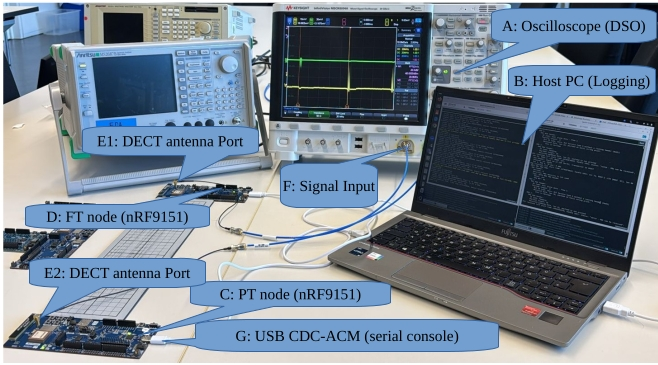
\includegraphics[width=1\linewidth]{main_setup.jpg}
\caption{Experimental setup for RX--TX turnaround measurements in \gls{nr}. Two nRF9151-based nodes are used (FT and PT). GPIO timing markers are connected to a \gls{dso} to measure the interval between RX completion and TX start. The RF port is terminated/controlled during timing measurements. Labels A--G indicate the main setup elements.}
\label{fig:setup}
\end{figure}

\subsection{Hardware Platform}

Experiments were conducted using two \gls{nr} nodes based on the Nordic Semiconductor nRF9151 system-on-chip. One node was configured as the \gls{nr} \gls{ft}, acting as the central controller, while the other node was configured as a \gls{pt}. The nRF9151 integrates the RF front-end, baseband processing, and protocol stack on a single device, and employs a single RF transceiver chain shared between reception and transmission.


\noindent\textbf{Host interface:} Each node is connected to the host laptop via USB (CDC-ACM) for logging and control (Linux device \texttt{/dev/ttyACM0}).
This hardware architecture prevents simultaneous  \gls{rx} and  \gls{tx} operation and requires explicit reconfiguration of the transceiver when switching between \gls{ul} and \gls{dl} communication. The nodes were operated using the \texttt{dect\_shell} \gls{nr} reference application, with minor instrumentation added to expose timing markers.

\subsection{Instrumentation and Timing Markers}

To obtain ground-truth timing measurements, GPIO signals were generated by the firmware to indicate key radio events. Specifically, GPIO markers were asserted upon completion of reception and upon initiation of transmission at the \gls{ft}. These signals were connected to a \gls{dso}, enabling direct measurement of the  \gls{rx}-- \gls{tx} turnaround delay.

In addition to external measurements, internal modem timing information was collected using firmware-accessible timers provided by the \gls{nr} modem. These timers report operation latencies in internal modem ticks and provide insight into radio state transitions and internal processing behavior.


\subsection{Measurement Procedure}

Measurements were performed under controlled conditions with minimal background traffic. The \glspl{ft} and \gls{pt} exchanged \gls{ul} and \gls{dl} traffic according to predefined scheduling patterns. For each experiment, multiple  \gls{rx}-- \gls{tx} transitions were captured to verify repeatability and consistency. The measured turnaround delay was extracted as the time difference between the  \gls{rx} completion marker and the  \gls{tx} start marker observed on the \gls{dso}.


\subsection{ \gls{rx}-- \gls{tx} Turnaround Measurement}

Fig.~\ref{fig:turnaround} illustrates the measured \gls{rx}--\gls{tx} turnaround process using GPIO timing markers captured on a digital storage oscilloscope. The yellow signal indicates the uplink transmission initiated by the \gls{pt}, during which the \gls{ft} is actively receiving. Once the uplink reception is completed, the \gls{ft} must reconfigure its transceiver from reception to transmission mode before it can respond. This reconfiguration results in a clearly observable idle interval between the end of the uplink transmission and the start of the downlink response. The measured \gls{rx}--\gls{tx} turnaround delay is approximately 850~\textmu s, corresponding to nearly two \gls{nr} slots. This delay is independent of the over-the-air transmission time and reflects the time required for transceiver reconfiguration, firmware processing, and alignment with the \gls{nr} frame structure.


Repeated measurements across multiple  \gls{rx}-- \gls{tx} transitions show consistent turnaround values with limited variation, indicating stable behavior under the considered operating conditions. The magnitude of the measured delay highlights that  \gls{rx}-- \gls{tx} switching constitutes a non-negligible component of the end-to-end latency in practical \gls{nr} systems.


\begin{figure}[t]
\centering
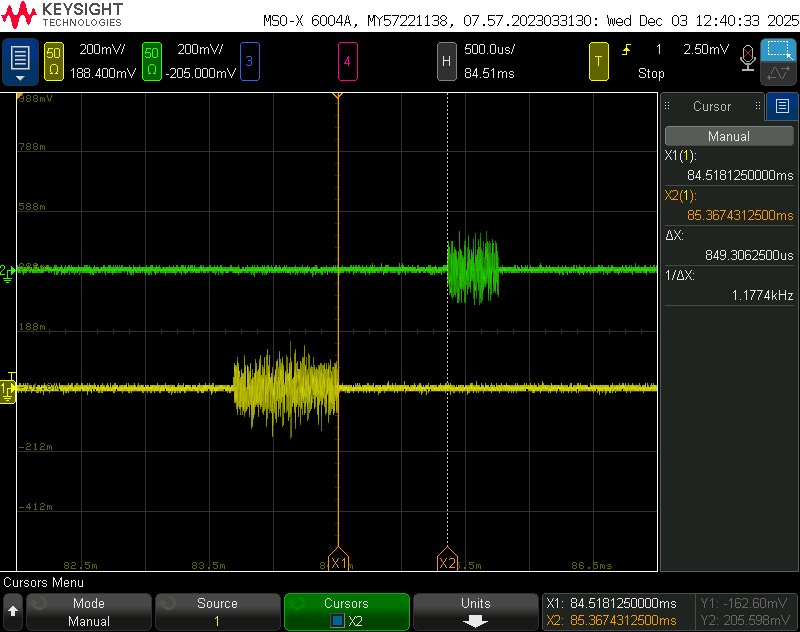
\includegraphics[width=0.95\linewidth]{osceliscope.jpg}
\caption{\gls{rx}--\gls{tx} turnaround behavior at the fixed termination (\gls{ft}). The yellow trace corresponds to the uplink transmission from the portable termination (\gls{pt}), during which the \gls{ft} operates in reception mode. After reception is completed, a distinct idle interval is observed before the \gls{ft} switches to transmission mode and sends the downlink response, indicated by the green trace. This idle interval represents the hardware- and firmware-induced \gls{rx}--\gls{tx} turnaround delay.
}
\label{fig:turnaround}
\end{figure}


\subsection{Cross-Validation Using Internal Modem Timing}

To further interpret the oscilloscope-based measurements, internal modem timing information was analyzed. The \gls{nr} modem reports operation latencies in internal modem ticks, where one slot corresponds to 28\,800 modem ticks. These timers capture the duration of internal radio state transitions and base-band processing steps, but do not represent the complete delay observable at the RF interface.

The reported modem latencies indicate that reception-related processing, including  \gls{rx} completion and RSSI handling, requires several hundred microseconds, while the  \gls{tx} start operation alone corresponds to approximately one \gls{nr} slot. When combined with firmware execution and slot-alignment effects, these internal timing values are consistent with the approximately 850~\textmu s turnaround delay measured using the oscilloscope. This agreement confirms that the observed turnaround latency is dominated by transceiver reconfiguration and scheduling-related effects rather than measurement artifacts.

\subsection{Latency Breakdown}

Based on the measurements, the total  \gls{rx}-- \gls{tx} turnaround latency can be conceptually decomposed into three main components: (i) internal  \gls{rx} processing and completion, (ii) transceiver reconfiguration and  \gls{tx} initiation, and (iii) firmware execution and alignment to the \gls{nr} slot structure. While the exact contribution of each component is implementation-dependent, the measurements indicate that no single component can be neglected when analyzing low-latency communication behavior.

%=============================Measurement Results and Scheduling Impact====================================================%

\section{Measurement Results and Scheduling Impact}

This section analyzes how \gls{ul} scheduling behavior interacts with the measured  \gls{rx}-- \gls{tx} turnaround delay and how this interaction affects end-to-end latency.

\subsection{Baseline Scheduling Behavior}

In the considered \gls{nr} implementation, \gls{ul} and \gls{dl} transmissions are scheduled sequentially using \gls{tdd}. Each change in transmission direction requires an  \gls{rx}-- \gls{tx} or  \gls{tx}-- \gls{rx} transition at the \gls{ft} or \gls{pt}, incurring the measured turnaround delay. As a result, the scheduling behavior directly determines how often this delay is incurred over time.

\subsection{Scheduling Scenarios}

To study the impact of scheduling on latency, two representative \gls{ul}-oriented scheduling scenarios are considered. In the first scenario, \gls{ul} transmissions are handled sequentially across frames, with each \gls{ul} transmission followed by an acknowledgment before the next transmission is scheduled. This behavior results in frequent \gls{ul}/\gls{dl} alternation and repeated turnaround delays.

In the second scenario, multiple \gls{ul} transmissions are grouped within a single frame, reducing frame boundary overhead. However, acknowledgment handling still requires frequent  \gls{rx}-- \gls{tx} switching, leading to accumulation of turnaround-induced latency.
\begin{figure*}[t]
\centering
\subfloat[Scenario~1: Sequential UL scheduling]{%
  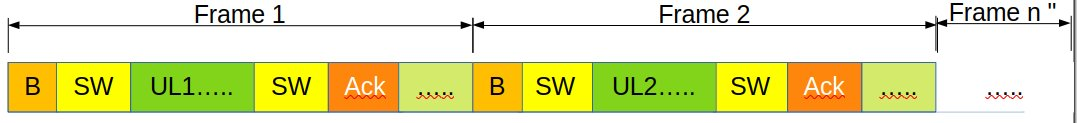
\includegraphics[width=0.48\textwidth]{scenario1.jpg}}
\hfill
\subfloat[Scenario~2: Grouped UL scheduling]{%
  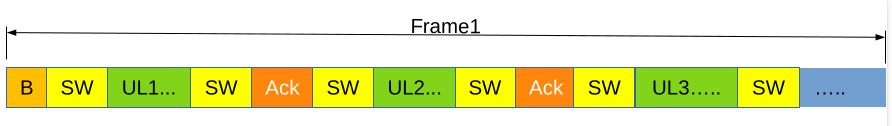
\includegraphics[width=0.48\textwidth]{scenario2.jpg}}

\vspace{0.3em}

\subfloat[Measured latency for Scenario~1]{%
  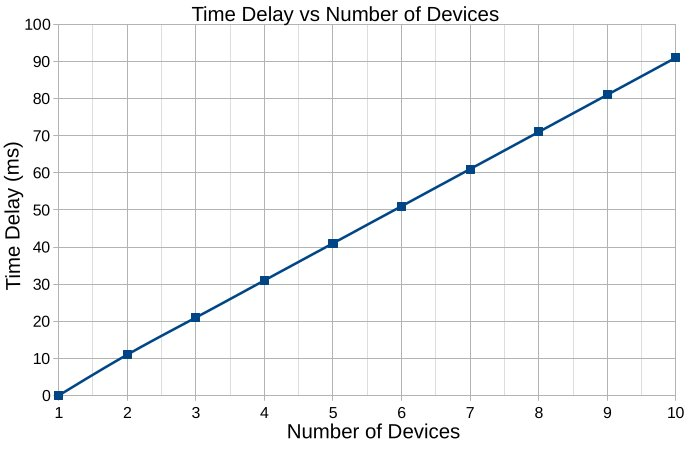
\includegraphics[width=0.48\textwidth]{s1graph.jpg}}
\hfill
\subfloat[Measured latency for Scenario~2]{%
  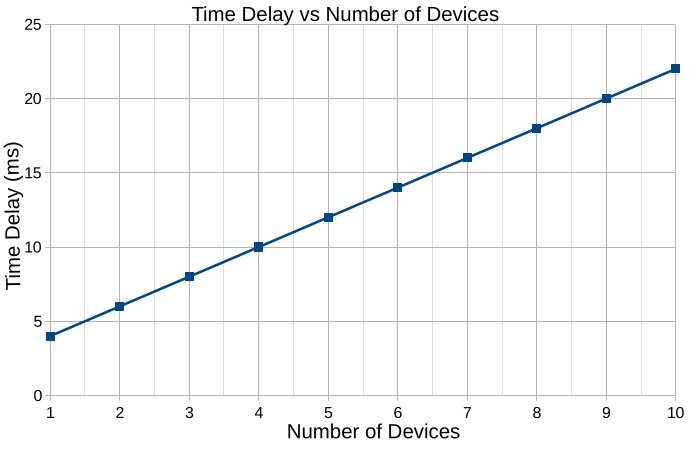
\includegraphics[width=0.48\textwidth]{s2graph.jpg}}

\caption{Scheduling scenarios and turnaround-induced latency. (a) Scenario~1: sequential \gls{ul} transmissions with an acknowledgment after each packet, causing frequent \gls{rx}--\gls{tx} switching within a separate frame. (b) Scenario~2: grouped \gls{ul} transmissions with acknowledgments scheduled after a batch in one frame. (c) Measured end-to-end latency as a function of the number of \gls{ul} transmissions for Scenario~1. (d) Corresponding latency measurements for Scenario~2.}
\label{fig:scheduling_latency}
\end{figure*}


Fig.~\ref{fig:scheduling_latency} shows the measured end-to-end latency as a function of the number of \gls{ul} transmissions for both scenarios. In both cases, latency increases approximately linearly with the number of \gls{ul} transmissions, indicating that  \gls{rx}-- \gls{tx} turnaround dominates the overall delay. While the second scenario reduces some scheduling overhead, the base latency remains high due to unavoidable direction switching on the single-transceiver platform.

These results demonstrate that scheduling strategies alone offer limited mitigation of turnaround-induced latency in practical \gls{nr} implementations. Significant latency reduction would require architectural changes that reduce or eliminate the need for frequent  \gls{rx}-- \gls{tx} switching.

%=============================Discussion, Design Implications, and Future Direction====================================================%

\section{Discussion, Design Implications, and Future Direction}

This section discusses the implications of the measurement results for \gls{ul}/\gls{dl} scheduling and hardware design in practical \gls{nr} systems. The focus is on understanding the fundamental limitations observed in the experiments and identifying directions for latency reduction beyond scheduling-level optimizations.

\subsection{Limits of Scheduling-Based Latency Reduction}

The results presented in the previous sections show that  \gls{rx}-- \gls{tx} turnaround delay constitutes a dominant component of end-to-end latency in the considered \gls{nr} implementation. Both oscilloscope measurements and internal modem timing indicate that each change in transmission direction incurs a delay on the order of multiple \gls{nr} slots. As a result, scheduling decisions that frequently alternate between \gls{ul} and \gls{dl} inherently accumulate significant latency.

The analysis of representative scheduling scenarios demonstrates that while grouping \gls{ul} transmissions can reduce some scheduling overhead, it does not eliminate the need for  \gls{rx}-- \gls{tx} switching when acknowledgments or \gls{dl} responses are required. Consequently, scheduling strategies alone offer limited potential for reducing latency in traffic patterns characterized by short packets or request--response behavior, which are common in industrial sensor--actuator applications.

\subsection{Impact on Industrial Sensor--Actuator Traffic}

In the considered sensor--actuator star topology, \gls{ul} sensor data and \gls{dl} actuator commands are tightly coupled in time. This asymmetry naturally leads to frequent \gls{ul}/\gls{dl} alternation at the \gls{ft}. The measured turnaround delay, therefore, directly affects control-loop latency and limits how quickly sensor information can be translated into actuator actions.

For such use cases, the observed latency is not primarily determined by physical-layer transmission time, but by the overhead associated with transceiver reconfiguration and scheduling alignment. This finding highlights the importance of considering hardware-induced delays when evaluating the suitability of \gls{nr} for low-latency industrial control applications.

\subsection{Architectural Considerations and Future Directions}

The measurement results presented in this work indicate that  \gls{rx}-- \gls{tx} turnaround delay is a dominant contributor to end-to-end latency in practical \gls{nr} systems employing single-transceiver hardware. This section discusses architectural considerations that arise from these findings and outlines potential directions for reducing turnaround-induced latency in future \gls{nr} implementations.

\subsubsection{Single-Transceiver Versus Multi-Chain Architectures}

The evaluated nRF9151-based platform employs a single RF transceiver chain shared between reception and transmission. While this architecture offers advantages in terms of cost, power consumption, and implementation complexity, it inherently requires sequential  \gls{rx} and  \gls{tx} operation. As shown by the oscilloscope measurements and modem timing analysis, the resulting  \gls{rx}-- \gls{tx} turnaround delay spans multiple \gls{nr} slots and cannot be eliminated through scheduling alone.

One architectural direction for reducing this limitation is the introduction of separate receive and transmit chains. Even partial separation, such as independent baseband processing with shared RF components, could reduce reconfiguration overhead and enable faster direction switching. However, such approaches introduce trade-offs related to hardware complexity, power consumption, and device cost, which must be carefully evaluated for industrial deployments.

\subsubsection{\gls{ul} and \gls{dl} Resource Separation}

Another potential approach to mitigating turnaround-induced latency is the separation of \gls{ul} and \gls{dl} resources in frequency or time. Allocating distinct channels for \gls{ul} and \gls{dl} communication could reduce or eliminate the need for frequent  \gls{rx}-- \gls{tx} switching at the \gls{ft}, particularly in sensor--actuator scenarios with tightly coupled request--response traffic.

While \gls{nr} primarily relies on \gls{tdd} to maximize spectral efficiency in unlicensed bands, future system designs could explore hybrid approaches that trade spectral efficiency for reduced latency in selected operating modes. Such mechanisms could be activated dynamically for latency-critical traffic, while preserving conventional \gls{tdd} operation for best-effort communication.

\subsubsection{Scheduling Awareness of Turnaround Costs}

The results of this study also suggest that scheduling decisions should explicitly account for hardware-induced turnaround costs. Rather than assuming negligible switching overhead, schedulers could incorporate turnaround-aware metrics when selecting transmission directions and grouping traffic. While such awareness cannot remove the turnaround delay itself on single-transceiver platforms, it may help avoid unnecessary direction changes and reduce latency accumulation under certain traffic patterns.

Importantly, the effectiveness of turnaround-aware scheduling is fundamentally bounded by the underlying hardware architecture. As demonstrated in this work, scheduling optimization alone offers limited gains when turnaround delays dominate the latency budget.

\subsubsection{Measurement-Driven System Design}

Finally, the combination of external oscilloscope measurements and internal modem timing analysis highlights the value of measurement-driven system design. External measurements provide ground-truth latency values observable at the RF interface, while internal timing information helps explain the origin of these delays. Future \gls{nr} system evaluations would benefit from similar multi-level measurement approaches to accurately characterize the interaction between hardware, firmware, and scheduling behavior.

Overall, the presented architectural considerations emphasize that achieving consistently low latency in \gls{nr} systems will likely require joint optimization across hardware architecture, duplexing strategy, and scheduling design, rather than relying on improvements at a single layer.

\section{Conclusion}

This paper presented a measurement-driven analysis of \gls{ul}/\gls{dl} scheduling and its impact on latency in \gls{nr} systems. Using oscilloscope-based timing measurements on an nRF9151-based platform, the  \gls{rx}-- \gls{tx} turnaround delay was quantified and shown to be on the order of two \gls{nr} slots. Internal modem timing information was used to cross-validate the external measurements and to provide insight into the underlying transceiver and firmware behavior.

The results demonstrated that  \gls{rx}-- \gls{tx} turnaround constitutes a dominant component of end-to-end latency in practical \gls{nr} implementations, particularly for short-packet and request--response traffic. Scenario-based analysis showed that while scheduling decisions influence how often this delay is incurred, scheduling alone offers limited potential for latency reduction on single-transceiver platforms. In industrial sensor--actuator use cases, frequent \gls{ul}/\gls{dl} alternation therefore leads to latency accumulation that cannot be mitigated purely at the scheduling level.

These findings highlight the importance of considering hardware-induced delays when evaluating low-latency \gls{nr} deployments. Future work will investigate architectural enhancements, such as \gls{ul}/\gls{dl} channel separation or parallel receive/transmit capabilities, and their potential to reduce turnaround-induced latency while preserving the flexibility and cost efficiency of \gls{nr} systems.


\bibliographystyle{IEEEtran}
\bibliography{Dectpaper}



\end{document}